\documentclass[8pt,xcolor=table,dvipsnames]{beamer}
\usepackage{pgfpages}
\usepackage{yhmath}
\newcommand{\Mod}[1]{\ (\mathrm{mod}\ #1)}
\providecommand{\half}{\frac{1}{2}}
\newcommand{\dg}{^\circ}
\newcommand{\arc}[1]{\wideparen{#1}}
\usetheme{Madrid}

\title{Geometric Transformations II}
\subtitle{UMC K1, 2024}
\author{Nghia Doan}
\institute{MCC Club \& Competitions}
\date{\today}

\begin{document}

\section{Rotations}

\begin{frame}[t]
    \frametitle{Geometric Transformations II}
    \framesubtitle{Rotations - Example 1}
    \begin{example}
        $P$ is an intersection point of circles $\omega_1$ and $\omega_2$.
        Construct a line through $P$ intersecting $\omega_1$ and $\omega_2$ at $A$ and $B$, respectively,
        such that $AP = PB.$
    \end{example}

    \begin{center}
        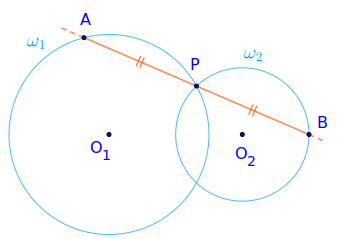
\includegraphics[width=5cm]{./svg/pdf/rotation-1a.pdf}
    \end{center}
\end{frame}

\begin{frame}[t]
    \frametitle{Geometric Transformations II}
    \framesubtitle{Rotations - Example 1}
    \begin{overprint}
        \onslide<1>Let \textbf{rotate} $\omega_2$ \textbf{half turn} ($180\dg$) or \textbf{reflect} $\omega_2$ \textbf{over point} $P$.
        Let $A$ be the other intersection of $\omega_1$ and the image of $\omega_1$ (the dotted circle); and $B$ be the intersection of $AP$ with $\omega_2.$
        \begin{center}
            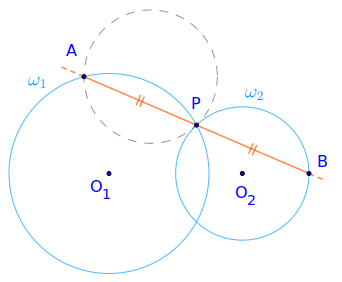
\includegraphics[width=5cm]{./svg/pdf/rotation-1b.pdf}
        \end{center}
        Then $A, P, B$ are collinear (why?) and $A$ is on the circumference of the image of $\omega_2$, thus $A$ is the image of $B$: $B \rightarrow A,$ thus $AP=BP.$
        \onslide<2>How many solutions?
        \begin{center}
            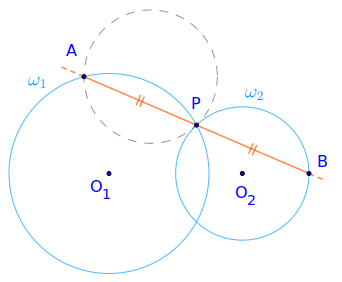
\includegraphics[width=5cm]{./svg/pdf/rotation-1b.pdf}
        \end{center}
        \begin{enumerate}
            \item If $|\omega_1 \cup \omega_2| = 2,$ then we have 1 solution.
            \item If $|\omega_1 \cup \omega_2| = 1,$ then we have no solution (why?)
            \item If $|\omega_1 \cup \omega_2| = 0,$ and the two radii are the same then we have infinitely many solutions
            otherwise no solution (why?).
        \end{enumerate}
    \end{overprint}    
\end{frame}

\begin{frame}[t]
    \frametitle{Geometric Transformations II}
    \framesubtitle{Rotations - Example 2}
    \begin{example}
        $P$ is an intersection point of circles $\omega_1$ and $\omega_2$.
        Construct a line through $P$ intersecting $\omega_1$ and $\omega_2$ at $A$ and $B$, respectively,
        such that $AP = 2PB.$
    \end{example}

    \begin{center}
        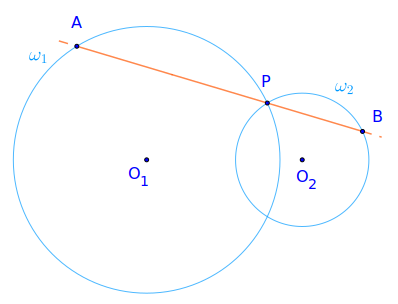
\includegraphics[width=5cm]{./svg/pdf/rotation-2a.pdf}
    \end{center}
\end{frame}

\begin{frame}[t]
    \frametitle{Geometric Transformations II}
    \framesubtitle{Rotations - Example 2}
    \onslide<1>The idea is \textbf{if $M$ is the midpoint of $AP$, then $\angle OMP = 90\dg$ and $MP = PB$}.
    Thus $M$ is the intersection of $\omega_2'$, the image of $\omega_2$ and the circle $\gamma$ diameter $O_1P.$
    \begin{center}
        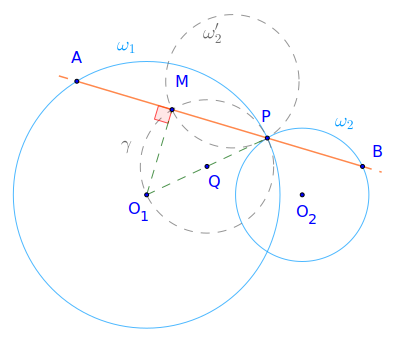
\includegraphics[width=5cm]{./svg/pdf/rotation-2b.pdf}
    \end{center}
    Thus we \textbf{rotate} $\omega_2$ \textbf{half turn} \textbf{over point} $P$.
    Then we draw the circle $\gamma$ diameter $O_1P.$
    Their intersection is $M$. Line through $MP$ intersects $\omega_1$ and $\omega_2$ at $A$ and $B$ respectively.
    \[
        AM \stackrel{OM \perp MP}{=} MP \stackrel{B \rightarrow M}{=} PB \Rightarrow AP = 2PB.
    \]
\end{frame}

\begin{frame}[t]
    \frametitle{Geometric Transformations II}
    \framesubtitle{Rotations - Example 3}
    \begin{example}
        $AB$ and $CD$ are chords of circle $\omega$. $J$ is a point on $CD$. Find point $X$ on the circumference of $\omega$ such that $JG = GF,$
        where $G$ and $F$ are intersections of $CD$ with $XA$ and $XB$, respectively.
    \end{example}

    \begin{center}
        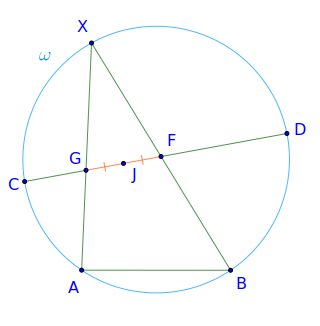
\includegraphics[width=5cm]{./svg/pdf/rotation-3a.pdf}
    \end{center}
\end{frame}

\begin{frame}[t]
    \frametitle{Geometric Transformations II}
    \framesubtitle{Rotations - Example 3}
    \begin{overprint}
        \onslide<1>The condition $GJ=JF$ give us the idea to \textbf{rotate} $X$ \textbf{half turn} \textbf{over point} $I$ to $X'$.
        \begin{center}
            \includegraphics[width=5cm]{./svg/pdf/rotation-3b.pdf}
        \end{center}
        Congruent triangles $\triangle XGJ$ and $\triangle XFJ$ shows that $\angle XGJ = \angle JFX,$ thus $FX' \parallel XA.$
        Furthermore $\angle X'FB = \angle AXB.$
        \onslide<2>We \textbf{rotate} $A$ \textbf{half turn} \textbf{over point} $I$ to $A'$.
        \begin{center}
            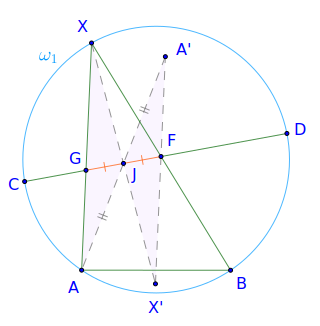
\includegraphics[width=5cm]{./svg/pdf/rotation-3c.pdf}
        \end{center}
        Therefore, $AXA'X'$ is a parallelogram.
        \onslide<3>$A'X'\parallel XA$ thus $X, F, A'$ are collinear.
        \begin{center}
            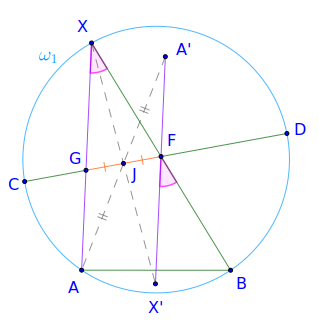
\includegraphics[width=5cm]{./svg/pdf/rotation-3d.pdf}
        \end{center}
        \onslide<4>$\angle A'FB = 180\dg - \angle F'XB = 180\dg - \angle AXB = 180\dg - \half \arc{AB}.$
        \begin{center}
            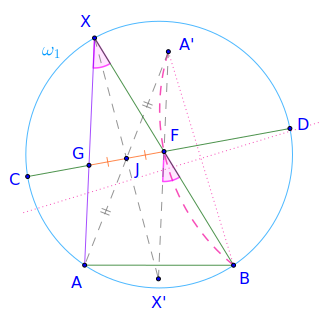
\includegraphics[width=5cm]{./svg/pdf/rotation-3e.pdf}
        \end{center}
        Hence, we first construct $A'$, then $F$ is the intersection the arc $\arc{A'B}$ with measure $180\dg - \half \arc{AB}$
        (how to construct an arc knowing the measure of the angle subtending it?) with the chord $CD.$
        Finally $X$ is the intersection of $BF$ with $\omega.$
    \end{overprint}
\end{frame}

\begin{frame}[t]
    \frametitle{Geometric Transformations II}
    \framesubtitle{Translations - Example 1}
    \begin{example}
        $n$ is a positive integer. Let $O_1, O_2, \ldots, O_{2n}$ be points on the plane and $AB$ is an arbitrary segment.
        Let segment $A_1B_1$ be obtained from $AB$ by half turn about $O_1$, let $A_2B_2$ be obtained from $A_1B_1$ by half turn about $O_2$, $\ldots,$
        and finally let $A_{2n}B_{2n}$ be obtained from $A_{2n-1}B_{2n-1}$ by half turn about $O_{2n}$ (see the figure for $n=2.$)

        \bigbreak
        Show that $AA_{2n} = BB_{2n}.$
    \end{example}

    \begin{center}
        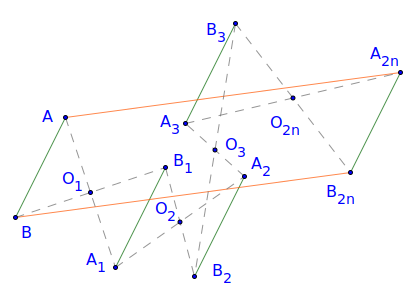
\includegraphics[width=5cm]{./svg/pdf/translation-1.pdf}
    \end{center}
\end{frame}

\begin{frame}[t]
    \frametitle{Geometric Transformations II}
    \framesubtitle{Translations - Example 1}
    \begin{overprint}
        \onslide<1>First, it is easy to see that \textbf{the sum of two half turns} around $O_1$ and $O_2$ is \textbf{a translation}:
        \[ 
            AA_2 \parallel BB_2 \parallel O_1O_2 \quad \text{and} \quad AA_2 = BB_2 = 2O_1O_2.
        \]
        \begin{center}
            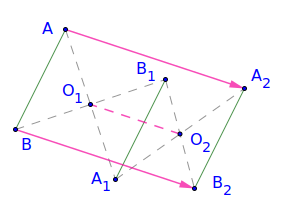
\includegraphics[width=5cm]{./svg/pdf/translation-1b.pdf}
        \end{center}
        \onslide<2>Thus, for an \textbf{even $2n$ number of translations, their sum is just another translation}, hence
        \[
            AA_{2n} = BB_{2n}.
        \]
        \begin{center}
            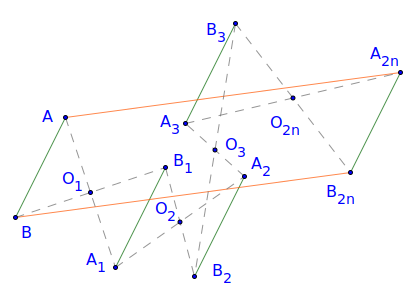
\includegraphics[width=5cm]{./svg/pdf/translation-1.pdf}
        \end{center}
    
        \bigbreak
        Is the conclusion still true if we have an \textbf{odd number of translations}? Why or why not?        
    \end{overprint}
\end{frame}

\begin{frame}[t]
    \frametitle{Geometric Transformations II}
    \framesubtitle{Translations - Example 2}
    \begin{example}
        $n$ is a positive odd integer. Let $O_1, O_2, \ldots, O_{n}$ be points on the plane.
        Let an arbitrary point $A$ be moved successively by half turns about $O_1, O_2, \ldots, O_{n}$
        and then once again moved successively by half turns about the same points $O_1, O_2, \ldots, O_{n}$.
        
        \bigbreak
        Show that the point $A_{2n}$, obtained as the result of these $2n$ half turns, coincides with the point $A.$
    \end{example}

    \begin{center}
        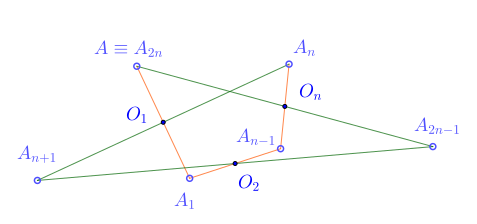
\includegraphics[width=5cm]{./svg/pdf/translation-2.pdf}
    \end{center}
\end{frame}

\begin{frame}[t]
    \frametitle{Geometric Transformations II}
    \framesubtitle{Translations - Example 2}
    Since the \textbf{sum of an odd number of half turns} is \textbf{a half turn}, the point $A_n$, obtained from $A$ by the $n$
    successive half turns about the points $O_1, O_2, \ldots, O_{n}$ can also be obtained from $A$ by a single half turn about some point $O$.
    \begin{center}
        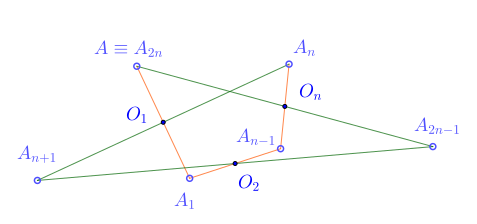
\includegraphics[width=5cm]{./svg/pdf/translation-2.pdf}
    \end{center}

    It is important to note that \textbf{$O$ depends on $O_1, O_2, \ldots, O_{n}$ only} and not $A$.
    
    \bigbreak
    The point $A_{2n}$ is obtained from $A_n$, by these same $n$ half turns;
    therefore it can also be obtained from $A_n$, by the single half turn about the point $O$.
    But this means that $A_{2n}$, coincides with $A$, because of the two half turns around the same point $O$.

    \bigbreak
    Is the conclusion still true if we have $n$ as \textbf{even number}? Why or why not?
\end{frame}

\begin{frame}[t]
    \frametitle{Geometric Transformations II}
    \framesubtitle{Translations - Example 3}
    \begin{example}
        $A_1A_2 \ldots A_{2n}$ is a $2n-$gon. $M_1, M_2, \ldots, M_{2n}$ are the midpoints of $A_1A_2,$ $A_2A_3,\ \ldots,$ $A_{2n}A_1$, respectively.
        Prove that there exists a $n-$gon whose sides are equal and parallel to the segments $M_1M_2,$ $M_3M_4,$ $\ldots$, $M_{2n-1}M_{2n}$
        and there exists a $n-$gon whose sides are equal and parallel to the segments $M_2M_3,$ $\ldots$, $M_{2n-2}M_{2n-1}$, $M_{2n}M_1.$ 
    \end{example}

    \begin{center}
        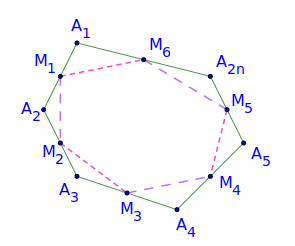
\includegraphics[width=5cm]{./svg/pdf/translation-3a.pdf}
    \end{center}
\end{frame}

\begin{frame}[t]
    \frametitle{Geometric Transformations II}
    \framesubtitle{Translations - Example 3}
    Note that by $2n$ half turns around $M_1, M_2, \ldots, M_{2n}$:
    \[
        A_1 \rightarrow A_2 \rightarrow A_3 \rightarrow  \cdots \rightarrow  A_{2n} \rightarrow A_1.
    \]
    
    The sum of two half turns around $M_1$ and $M_2$ is a translation $A_1 \rightarrow A_3$ with distance $A_1A_3 = 2 M_1M_2$
    similarly the sum of two half turns around $M_3$ and $M_4$ is a translation $A_3 \rightarrow A_5$ with distance $A_3A_4 = 2 M_3M_4$
    and so on.

    \begin{center}
        \includegraphics[width=5cm]{./svg/pdf/translation-3b.pdf}
    \end{center}

    Furthermore after $n$ translations: $A_1 \rightarrow A_1,$ therefore the sum of them is an \textbf{identity transformation},
    thus the $n$ translations form a \textbf{close path} and therefore is an $n-$gon.

    \bigbreak
    Hence, each of the sides is equal and parallel to the segments $M_1M_2,$ $M_3M_4,$ $\ldots$, $M_{2n-1}M_{2n}$.
\end{frame}

\begin{frame}[t]
    \frametitle{Geometric Transformations II}
    \framesubtitle{Translations - Example 3}
    \begin{example}
        $A_1A_2 \ldots A_{2n}$ is a $2n-$gon. $M_1, M_2, \ldots, M_{2n}$ are the midpoints of $A_1A_2,$ $A_2A_3,\ \ldots,$ $A_{2n}A_1$, respectively.
        Prove that there exists a $n-$gon whose sides are equal and parallel to the segments $M_1M_2,$ $M_3M_4,$ $\ldots$, $M_{2n-1}M_{2n}$
        and there exists a $n-$gon whose sides are equal and parallel to the segments $M_2M_3,$ $\ldots$, $M_{2n-2}M_{2n-1}$, $M_{2n}M_1.$ 
    \end{example}

    \begin{center}
        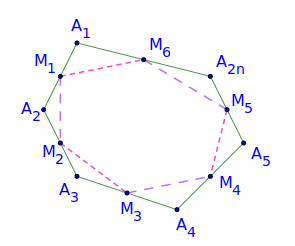
\includegraphics[width=5cm]{./svg/pdf/translation-3a.pdf}
    \end{center}
\end{frame}

\begin{frame}[t]
    \frametitle{Geometric Transformations II}
    \framesubtitle{Translations - Example 3}
    Note that by $2n$ half turns around $M_1, M_2, \ldots, M_{2n}$:
    \[
        A_1 \rightarrow A_2 \rightarrow A_3 \rightarrow  \cdots \rightarrow  A_{2n} \rightarrow A_1.
    \]
    
    The sum of two half turns around $M_1$ and $M_2$ is a translation $A_1 \rightarrow A_3$ with distance $A_1A_3 = 2 M_1M_2$
    similarly the sum of two half turns around $M_3$ and $M_4$ is a translation $A_3 \rightarrow A_5$ with distance $A_3A_4 = 2 M_3M_4$
    and so on.

    \begin{center}
        \includegraphics[width=5cm]{./svg/pdf/translation-3b.pdf}
    \end{center}

    Furthermore after $n$ translations: $A_1 \rightarrow A_1,$ therefore the sum of them is an \textbf{identity transformation},
    thus the $n$ translations form a \textbf{close path} and therefore is an $n-$gon.

    \bigbreak
    Hence, each of the sides is equal and parallel to the segments $M_1M_2,$ $M_3M_4,$ $\ldots$, $M_{2n-1}M_{2n}$.
\end{frame}

\begin{frame}[t]
    \frametitle{Geometric Transformations II}
    \framesubtitle{Rotations - Example 4}
    \begin{example}
        Three parallel lines $\ell_1$, $\ell_2,$ and $\ell_3$ are given. $A$ is a point on the line $\ell_1$.
        
        \bigbreak
        How can we determine points $B$ and $C$ on $\ell_2$ and $\ell_3$, respectively, such that $ABC$ is an equilateral triangle.
    \end{example}

    \begin{center}
        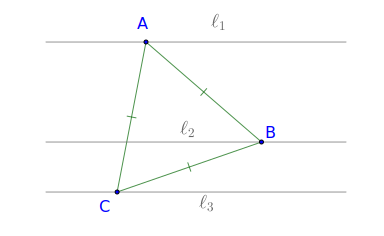
\includegraphics[width=5cm]{./svg/pdf/rotation-4a.pdf}
    \end{center}
\end{frame}

\begin{frame}[t]
    \frametitle{Geometric Transformations II}
    \framesubtitle{Rotations - Example 4}
    \begin{overprint}
        \onslide<1>Assume that $\triangle ABC$ is equilateral, then \textbf{a rotation by $60\dg$ about $A$ will carry $B$ to $C$}.
        \begin{center}
            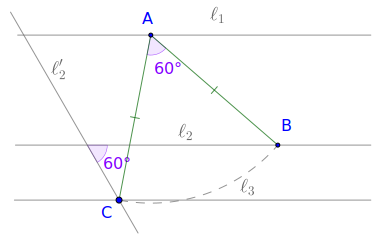
\includegraphics[width=5cm]{./svg/pdf/rotation-4b.pdf}
        \end{center}
        That rotation also carries $\ell_2$  (containing $B$) to $\ell_2'$. The intersection of $\ell_2'$ and $\ell_3$ is $C.$
        \onslide<2>Now we know how to do it. Rotate $\ell_2$ by $60\dg$ about $A$ to obtain $\ell_2'$.
        The intersection of $\ell_2'$ with $\ell_3$ is the position for $C.$
        $B$ can be constructed easily as the intersection of circle centred at $A$ radius $AC.$
        \begin{center}
            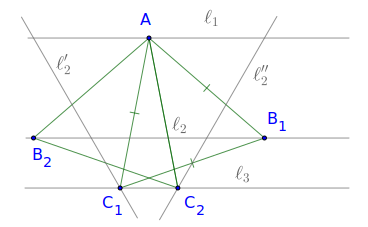
\includegraphics[width=5cm]{./svg/pdf/rotation-4c.pdf}
        \end{center}
    
        \bigbreak
        Note that there are two different solutions (why?)
    \end{overprint}
\end{frame}

\begin{frame}[t]
    \frametitle{Geometric Transformations II}
    \framesubtitle{Rotations - Example 5}
    \begin{example}
        Three concentric circles $\omega_1$, $\omega_2,$ and $\omega_3$ are given. $A$ is a point on the line $\omega_1$.
        
        \bigbreak
        How can we determine points $B$ and $C$ on $\omega_2$ and $\omega_3$, respectively, such that $ABC$ is an equilateral triangle.
    \end{example}

    \begin{center}
        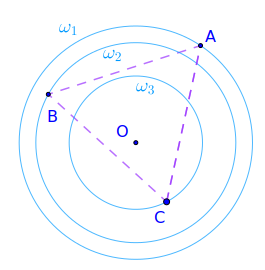
\includegraphics[width=5cm]{./svg/pdf/rotation-5a.pdf}
    \end{center}
\end{frame}

\begin{frame}[t]
    \frametitle{Geometric Transformations II}
    \framesubtitle{Rotations - Example 4}
    Pretty much the same as in the solution for the previous example.
    
    \bigbreak
    Rotate $\omega_2$ by $60\dg$ about $A$ to obtain $\omega_2'$.
    The intersection of $\omega_2'$ with $\omega_3$ is the position for $C.$
    $B$ can be constructed easily as the intersection of circle centred at $A$ radius $AC.$
    \begin{center}
        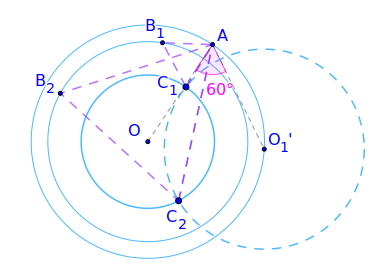
\includegraphics[width=5cm]{./svg/pdf/rotation-5b.pdf}
    \end{center}

    \bigbreak
    Note that there are \textbf{at most four} different solutions (why?).
\end{frame}

\begin{frame}[t]
    \frametitle{Geometric Transformations II}
    \framesubtitle{Rotations - Example 6}
    \begin{example}
        On the sides of an arbitrary triangle $ABC,$ exterior to it, construct isosceles triangles $BCA_1$ $ACB_1$, $CAB_1$
        with angles at the vertices $A_1$, $B_1$, and $C_1$, respectively equal to $\alpha$, $\beta$ and $\gamma$.
        \bigbreak
        Prove that if $\alpha + \beta + \gamma = 360\dg$, then the angles of the triangle $A_1B_1C_1$
        are equal to $\half\alpha$, $\half\beta$ and $\half\gamma$, that is, they do not depend on the shape of the triangle $ABC.$
    \end{example}

    \begin{center}
        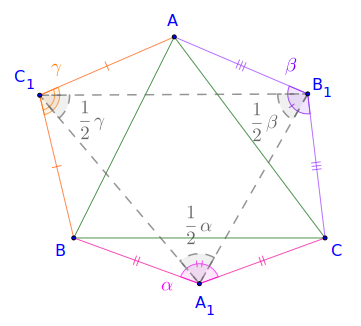
\includegraphics[width=5cm]{./svg/pdf/rotation-6a.pdf}
    \end{center}
\end{frame}

\begin{frame}[t]
    \frametitle{Geometric Transformations II}
    \framesubtitle{Sum of Rotations}
    \begin{overprint}
        \onslide<1>Let's take a look at a \textbf{sum of two rotations}:
        \[
            AB \stackrel{\text{rotate}(O_1, \alpha)}{\rightarrow} A_1B_1 \stackrel{\text{rotate}(O_2, \beta)}{\rightarrow} A_2B_2.
        \]
        \begin{center}
            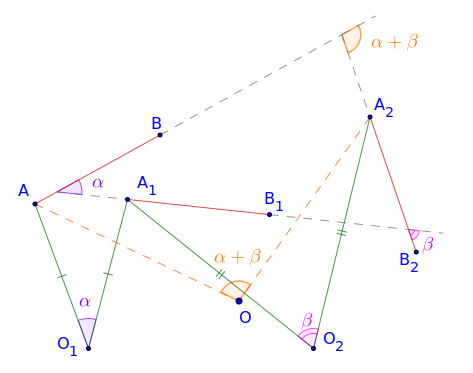
\includegraphics[width=5cm]{./svg/pdf/sum-rotations-1.pdf}
        \end{center}

        It is easy to see that the angle between $A_2B_2$ and $AB$ is $\alpha + \beta$, thus it is a rotation by the angle $\alpha + \beta,$
        We need to determine the position of the center of rotation $O$.
        \onslide<2>Now, what happen with the centers $O_1$ and $O_2$:
        \[
            O_1 \stackrel{\text{rotate}(O_1, \alpha)}{\rightarrow} O_1 \stackrel{\text{rotate}(O_2, \beta)}{\rightarrow} O_1'
            \quad \text{and} \quad O_2'' \stackrel{\text{rotate}(O_1, \alpha)}{\rightarrow} O_2 \stackrel{\text{rotate}(O_2, \beta)}{\rightarrow} O_2.
        \]
        \begin{center}
            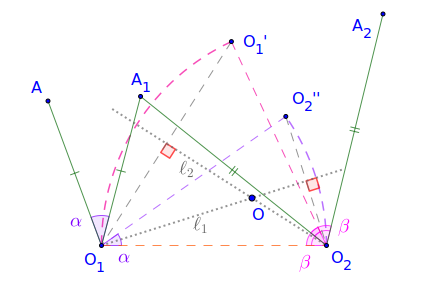
\includegraphics[width=5cm]{./svg/pdf/sum-rotations-2.pdf}
        \end{center}
        Therefore $O$ is on both perpendicular bisectors of $O_1O_1'$ and $O_2''O_2$.

        \bigbreak        
        Hence, $\angle OO_1O_2 = \half \alpha,$  $\angle OO_2O_1 = \half \beta.$
    \end{overprint}
\end{frame}

\begin{frame}[t]
    \frametitle{Geometric Transformations II}
    \framesubtitle{Rotations - Example 6}
    \begin{overprint}
        \onslide<1>First, point $A$ is taken into itself by the sum of three rotations through the angles $\beta$, $\alpha$, and $\gamma$
        ($\alpha + \beta + \gamma = 360\dg$) about the centers $B_1, A_1, C_1$:
        \[
            A \stackrel{\text{rotate}(B_1, \beta)}{\rightarrow} C \stackrel{\text{rotate}(A_1, \alpha)}{\rightarrow} B 
            \stackrel{\text{rotate}(C_1, \gamma)}{\rightarrow} A. 
        \]
        \begin{center}
            \includegraphics[width=5cm]{./svg/pdf/rotation-6b.pdf}
        \end{center}
        Thus, the \textbf{sum of the these rotations} is the \textbf{identity transformation}.
        \onslide<2>Let $C'$ be the center of the rotation equivalent to the sum of the rotations about $B_1$ and $A_1$.
        Then it is the rotation through $\alpha + \beta = 360\dg - \gamma$ brings $A$ to $B$.
        \bigbreak
        However, the rotation about $C_1$ through $\gamma$ brings $A$ to $B$ in opposite direction.
        Since a rotation through an angle $\theta$ is the same as the rotation through an angle $360\dg - \theta$
        about the same center in the opposite direction, thus $C_1 \equiv C'.$
        \begin{center}
            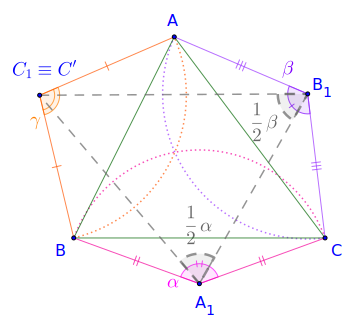
\includegraphics[width=5cm]{./svg/pdf/rotation-6c.pdf}
        \end{center}
        Therefore $\angle C_1A_1B_1 = \half \alpha, \angle C_1B_1A_1 = \half \beta,$ and similarly $\angle B_1C_1A_1 = \half \gamma.$ 
    \end{overprint}
\end{frame}

\begin{frame}[t]
    \frametitle{Geometric Transformations II}
    \framesubtitle{Symmetry - Example 1}
    \begin{example}
        $\angle MON$ is given, together with two points $A$ and $B$.
        Find a point $X$ on the side $OM$ such that the triangle $XYZ$ is isosceles: $XY = XZ$, 
        where $Y$ and $Z$ are on the points of intersection of $XA$ and $XB$ with $ON.$ 
    \end{example}

    \begin{center}
        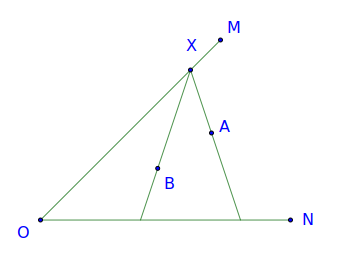
\includegraphics[width=5cm]{./svg/pdf/symmetry-1a.pdf}
    \end{center}
\end{frame}

\begin{frame}[t]
    \frametitle{Geometric Transformations II}
    \framesubtitle{Symmetry - Example }
    Let $B'$ be the image of $B$ over $OM,$ then:
    \[
        \angle B'XA = \angle B'XB + \angle YXZ,\  \angle B'XB = 2\angle OXZ = 2(\angle XZY - \angle MON)
        \Rightarrow \angle B'XA = 180\dg - \angle MON.
    \]

    \begin{center}
        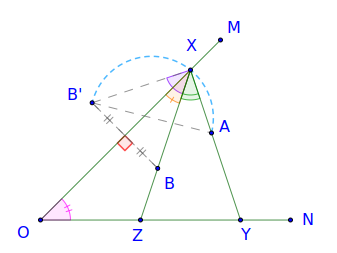
\includegraphics[width=5cm]{./svg/pdf/symmetry-1b.pdf}
    \end{center}
    Thus, $X$ is the intersection of $OM$ with the arc constructed on the chord $AB',$ that subtends an angle equal to $180\dg - \angle MON.$
\end{frame}

\begin{frame}[t]
    \frametitle{Geometric Transformations II}
    \framesubtitle{Symmetry - Example 2}
    \begin{example}
        Construct a quadrilateral $ABCD$ in which a circle can be inscribed,
        given the lengths of two adjacent sides $AB$ and $AD$ and the angles at the vertices $B$ and $D.$
    \end{example}

    \begin{center}
        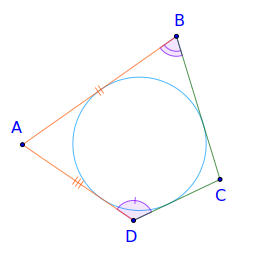
\includegraphics[width=5cm]{./svg/pdf/symmetry-2a.pdf}
    \end{center}
\end{frame}

\begin{frame}[t]
    \frametitle{Geometric Transformations II}
    \framesubtitle{Symmetry - Example 2}
    \begin{overprint}
        \onslide<1>The key idea here is that the reflection of $CD$ over the line through $A$ and the center of the circle is a tangent to the circle!
        \begin{center}
            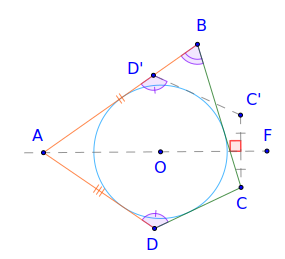
\includegraphics[width=5cm]{./svg/pdf/symmetry-2d.pdf}
        \end{center}
        \onslide<2>First, we start the construction by point $A$ then segment $AB$,
        then segment $AD_1 = AD$ where $D$ is on the line $AB,$ same side as $B$ in respect to $A$.

        \bigbreak
        Second, because $\angle B$ and $\angle D_1= \angle D$ are known, thus we can construct rays going from $B$ and $D_1.$
        
        \bigbreak
        Finally, we construct a circle tangents to all three lines.
        \begin{center}
            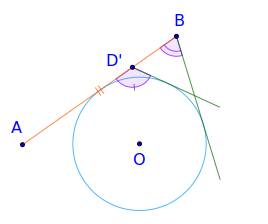
\includegraphics[width=5cm]{./svg/pdf/symmetry-2b.pdf}
        \end{center}
        \onslide<3>The rest is simple, we reflect $D'$ and its ray over the line $AO$ where $O$ is the center of the circle.
        The reflected ray will intersect the ray from $B$ at $C.$ We are done.
        \begin{center}
            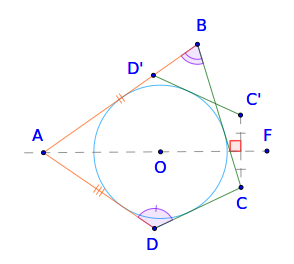
\includegraphics[width=5cm]{./svg/pdf/symmetry-2c.pdf}
        \end{center}
    \end{overprint}
\end{frame}

\begin{frame}[t]
    \frametitle{Geometric Transformations II}
    \framesubtitle{Symmetry - Example 3}
    \begin{example}
        \textit{A billiard ball bounces off a side of a billiard table in such a manner that the two lines along
        which it moves before and after hitting the sides are equally inclined to the side.}

        Suppose a billiard table were bordered by $n$ lines $\ell_1, \ell_2, \ldots, \ell_n$.
        Let $A$ and $B$ be two given points on the billiard table.
        In what direction should one hit a ball placed at $A$
        so that it will bounce consecutively off the lines $\ell_1, \ell_2, \ldots, \ell_n$,
        and then pass through the point $B$ (see the diagram below, where $n = 3$)?
    \end{example}

    \begin{center}
        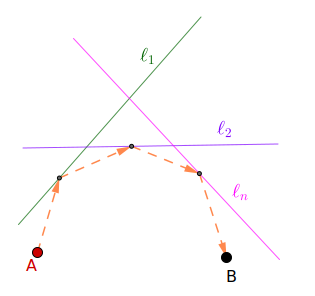
\includegraphics[width=4cm]{./svg/pdf/symmetry-3a.pdf}
    \end{center}
\end{frame}

\begin{frame}[t]
    \frametitle{Geometric Transformations II}
    \framesubtitle{Symmetry - Example 3}
    Assume that the problem has been solved, that is, that points
    $X_1, X_2, \ldots X_n$ have been found on the lines $\ell_1, \ell_2, \ldots, \ell_n$ such that
    $A X_1 X_2 \cdots X_n B$ is the path of a billiard ball (the case $n = 3$).
    \begin{center}
        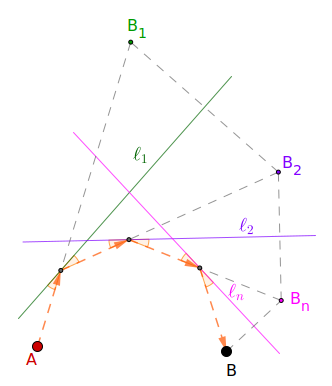
\includegraphics[width=3.5cm]{./svg/pdf/symmetry-3b.pdf}
    \end{center}
    \begin{overprint}
        \onslide<1>It is easy to see that the point $X_n$, is the point of intersection of the line $\ell_n$ with the line $X_{n-1}B_n$,
        where $B_n$, is the image of $B$ in $\ell_n$, that is, the points $B_n$,$X_n$, $X_{n-1}$ lie on a line.
        \bigbreak
        But then the point $X_{n-1}$ is the point of intersection of the line $\ell_{n-1}$ with the $X_{n-2}B_{n-1}$,
        where $B_{n-1}$, is the image of $B_n$ in $\ell_{n-1}$ and so on.
        \onslide<2>Here's the construction: Reflect the point $B$ in $l_n$, obtaining the point $B_n$;
        next reflect $B_n$ in $l_{n-1}$ to obtain $B_{n-1},$ and so forth, until the image $B_1$ of the point $B_2$, in line $\ell_1$ is obtained.
        \bigbreak
        The point $X_1$, that determines the direction in which the billiard ball at $A$ must be hit,
        is obtained as the point of intersection of the line $\ell_1$ with the line $AB_1$.
        It is then easy to find the points $X_2, \ldots X_n$ with the aid of the points $B_2, \ldots B_n$ and $X_1$.
    \end{overprint}
\end{frame}

\end{document}
